%%%%%%%%%%%%%%%%%%%%%%%%%%%%%%%%%%%%%%%%%
% baposter Landscape Poster
% LaTeX Template
% Version 1.0 (11/06/13)
%
% baposter Class Created by:
% Brian Amberg (baposter@brian-amberg.de)
%
% This template has been downloaded from:
% http://www.LaTeXTemplates.com
%
% License:
% CC BY-NC-SA 3.0 (http://creativecommons.org/licenses/by-nc-sa/3.0/)
%
%%%%%%%%%%%%%%%%%%%%%%%%%%%%%%%%%%%%%%%%%

%----------------------------------------------------------------------------------------
%	PACKAGES AND OTHER DOCUMENT CONFIGURATIONS
%----------------------------------------------------------------------------------------
%0.285
\documentclass[landscape,a2paper,fontscale=1]{baposter} % Adjust the font scale/size here

\usepackage{xcolor}
\usepackage{graphicx} % Required for including images
\graphicspath{{figures/}} % Directory in which figures are stored

\usepackage{amsmath} % For typesetting math
\usepackage{amssymb} % Adds new symbols to be used in math mode

\usepackage{booktabs} % Top and bottom rules for tables
\usepackage{enumitem} % Used to reduce itemize/enumerate spacing
\usepackage{palatino} % Use the Palatino font
\usepackage[font=small,labelfont=bf]{caption} % Required for specifying captions to tables and figures

\usepackage{multicol} % Required for multiple columns
\usetikzlibrary{shapes,arrows} % Tikz libraries required for the flow chart in the template

\newcommand{\compresslist}{ % Define a command to reduce spacing within itemize/enumerate environments, this is used right after \begin{itemize} or \begin{enumerate}
\setlength{\itemsep}{1pt}
\setlength{\parskip}{0pt}
\setlength{\parsep}{0pt}
}

\definecolor{lightblue}{rgb}{0.145,0.6666,1} % Defines the color used for content box headers

\begin{document}

\background{%
    \begin{tikzpicture}
        [remember picture,overlay]\node[opacity=1] at (current page.center) {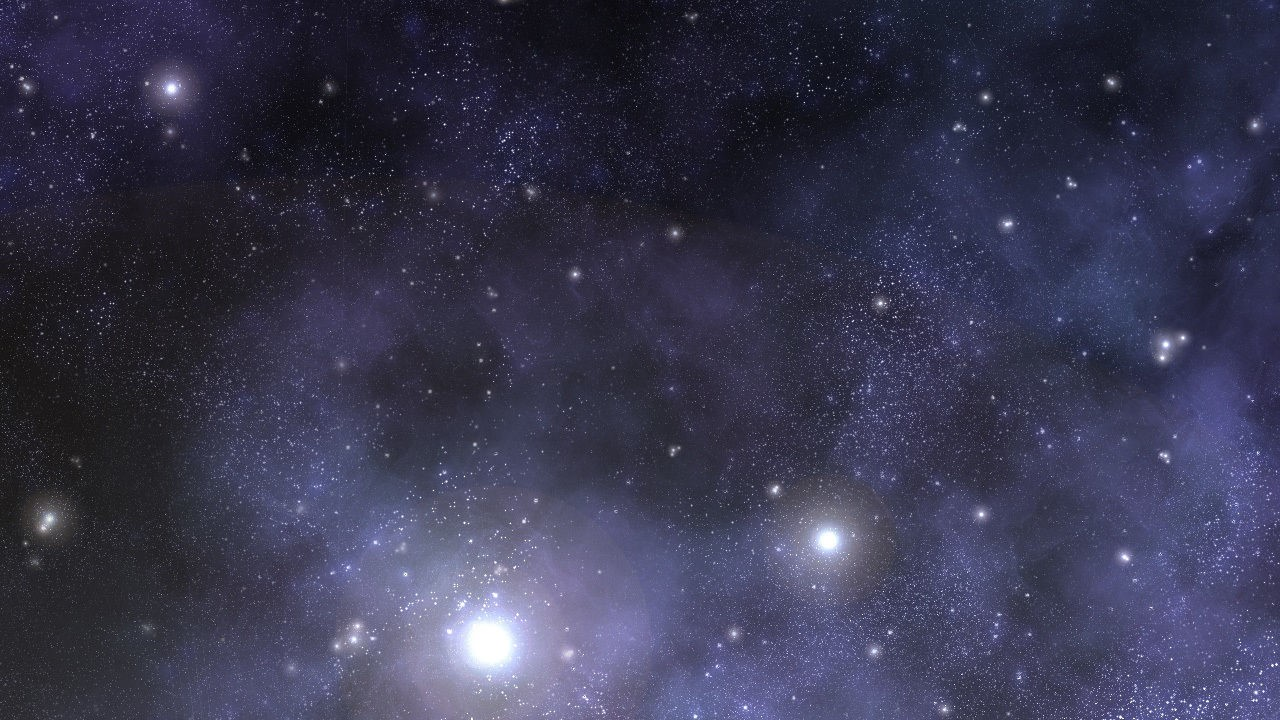
\includegraphics[width=\paperwidth,height=\paperheight]{star-field-space-background-3d-model}};
    \end{tikzpicture}%
}

\begin{poster}
{
headerborder=closed, % Adds a border around the header of content boxes
colspacing=1em, % Column spacing
%bgColorOne=white, % Background color for the gradient on the left side of the poster
%bgColorTwo=white, % Background color for the gradient on the right side of the poster
borderColor=lightblue, % Border color
headerColorOne=black, % Background color for the header in the content boxes (left side)
headerColorTwo=lightblue, % Background color for the header in the content boxes (right side)
headerFontColor=white, % Text color for the header text in the content boxes
boxColorOne=white, % Background color of the content boxes
textborder=roundedleft, % Format of the border around content boxes, can be: none, bars, coils, triangles, rectangle, rounded, roundedsmall, roundedright or faded
eyecatcher=true, % Set to false for ignoring the left logo in the title and move the title left
headerheight=0.1\textheight, % Height of the header
headershape=roundedright, % Specify the rounded corner in the content box headers, can be: rectangle, small-rounded, roundedright, roundedleft or rounded
headerfont=\Large\bf\textsc, % Large, bold and sans serif font in the headers of content boxes
%textfont={\setlength{\parindent}{1.5em}}, % Uncomment for paragraph indentation
background=user,
linewidth=2pt % Width of the border lines around content boxes
}
%----------------------------------------------------------------------------------------
%	TITLE SECTION 
%----------------------------------------------------------------------------------------
%
{
\includegraphics[height=8em]{DUlogo.png}} % First university/lab logo on the left
{\bf\textcolor{white}{\textsc{Modelling Rotating Black Holes}\vspace{0.5em}}} % Poster title
{\textcolor{white}{\textsc{ Joseph Sweeney \hspace{12pt} Supervised by Kasper Peeters}}} % Author names and institution
{
\includegraphics[height=8em]{DUlogo.png}} % Second university/lab logo on the right

%----------------------------------------------------------------------------------------
%	REFERENCES
%----------------------------------------------------------------------------------------

\headerbox{References}{name=references,column=0,span=4,above=bottom}{
\renewcommand{\section}[2]{\vskip 0.05em} % Get rid of the default "References" section title
\nocite{*} % Insert publications even if they are not cited in the poster
\small{ % Reduce the font size in this block
\begin{multicols}{2}
\bibliographystyle{unsrt}
\bibliography{sample} % Use sample.bib as the bibliography file
\end{multicols}
}}
%----------------------------------------------------------------------------------------
%	Introduction
%----------------------------------------------------------------------------------------

\headerbox{1. Black Holes}{name=introduction,column=0,row=0}{

Since the release of the blockbuster film Interstellar, and more recently, the first successful imaging of a black holes shadow; interest in the field of modelling black holes has significantly risen. There are many methods one can use to model black holes, and some tricks to improve computation. This poster will outline what I have learnt while researching this extraordinary field.

\vspace{1em}

Though black holes are remarkably complex, the No-Hair Theorem states that they are defined entirely by only three parameters - mass, spin and charge. All black holes must have non-zero mass inherently, but the addition of charge and spin can change the properties significantly (for example a black hole with zero spin has spherical symmetry). However the inclusion of non-zero spin removes this symmetry, making equations of motion in the metric defining the black hole much more complex. Here is a table of the most commonly used metrics to describe each kind of black hole:

\vspace{1em}
\begin{center}
\begin{tabular}{l l l}
\toprule
\textbf{ } & \textbf{Spin} & \textbf{No Spin}\\
\midrule
\textbf{Charge} & Kerr-Newman & Reissner-Nordström \\
\midrule
\textbf{No Charge} & Kerr & Schwarzschild \\
\bottomrule
\end{tabular}
\captionof{table}{Metrics to describe black holes}
\end{center}

\vspace{1em}
Of course, one could use the  Kerr-Newman metric and simply take spin and/or charge to be zero and it would be equivalent to one of the other metrics, so objectively this is the most useful and general metric. However, if we know that we are uninterested in one of the variables it creates more work for us to abstract our work to allow for changing this variable.

\vspace{1em}
We are particularly interested in the Kerr metric; which can describe a rotating, non-charged black hole. A Kerr black hole has spin parameter per unit mass J = $\frac{a}{M}$, where M is the mass of the black hole and a is a the spin parameter. J can range from 0 (describing a Schwarzschild black hole) to 1 (an extreme Kerr black hole). When J is taken to be greater than one, the Kerr metric can be used to describe a naked singularity, which is a singularity with no event horizon surrounding it.
}

%----------------------------------------------------------------------------------------
%	The Schwarzschild Metric
%----------------------------------------------------------------------------------------

\headerbox{2. The Schwarzschild Metric}{name=schwarzschild,column=1,span=2,row=0, bottomaligned=introduction}{ % This block's bottom aligns with the bottom of the conclusion block
\begin{multicols}{2}
The Schwarzschild metric is given in line notation by:

\begin{equation}
{ds^{2} = {\left(1-\frac {2M}{r}\right)}^{-1}} {dr^2} + {r^2}{d\varphi ^2} -{\left(1-\frac {2M}{r}\right)}{dt^2}
\end{equation}\

Note that due to the spherical symmetry of the Schwarzschild metric, here we have taken $\theta=\frac{\pi}{2}$ which simplifies the metric. By using Hamiltonians formalisation on the metric, we can derive equations of motion for light-like (or null) particles in the metric:

\begin{equation}
\ddot{r} = -\frac{L^2(3M-r)}{r^4}
\end{equation}
\[\dot{\varphi}=\frac{L}{r^2}\]

By solving these coupled differential equations numerically, and keeping track of relevant variables, we have all the elements needed to plot the path of a photon in the Schwarzschild metric. You can see a plot similar to this for the Kerr metric in Figure 3.

\vspace{1em}
We are interested in the angle between the line from our starting point, to the final position of the photon (assuming the photon did not cross the event horizon), and the line from our starting point to the centre of the black hole. Using some simple geometry and our final position, we may find this given our launch angle.

\vspace{1em}
As we have taken $\theta=\frac{\pi}{2}$, we are working in two dimensions, so we may run this program along launch angles from $-\frac{\pi}{2}\mbox{ to }\frac{\pi}{2}$ and find a function relating launch angle to final angle. Here we run only in this region, and not inclusive at the minimum and maximum angles as doing otherwise leads to division by zero in our code when calculating initial conditions required to give launch angle.

\vspace{1em}
If a pixel leads to the calculation being cut off, we know that the photon has entered the event horizon, so we colour the current pixel in black. Elsewise, we may calculate the required launch angle for a photon to reach this pixel in ordinary spacetime, and using the function of launch angle find the final angle of the photon. 

\vspace{1em}
To create a coherant image of the shadow of a Schwarzschild black hole, we must first consider what taking $\theta=\frac{\pi}{2}$ means to us. Since we are embedding into two dimensions, this means that for an initial pixel on an image, the possible final positions on the image has been embedded from 2-d (the image), to 1-d (a line passing through the inital pixel and the centre of the image).

\vspace{1em}
 We could visualise the process of generating an image as taking a straight line through the centre of a background image, and for each pixel on this line finding the necessary launch angle, running our code, and finding final angle. Then, using the direct correspondance between length and angle, find where along the line the final position of the photon is (see Figure 1, left). This will generate a line of pixels, so we rotate this line about the centre of the image until we have formed a generated circle.

\begin{center}
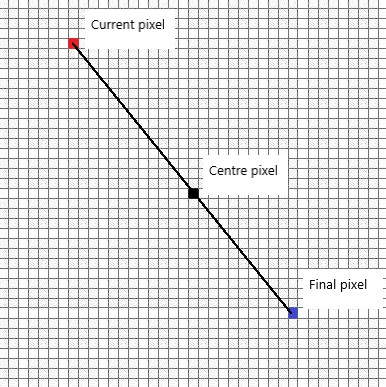
\includegraphics[height=0.45\linewidth]{grid-final}
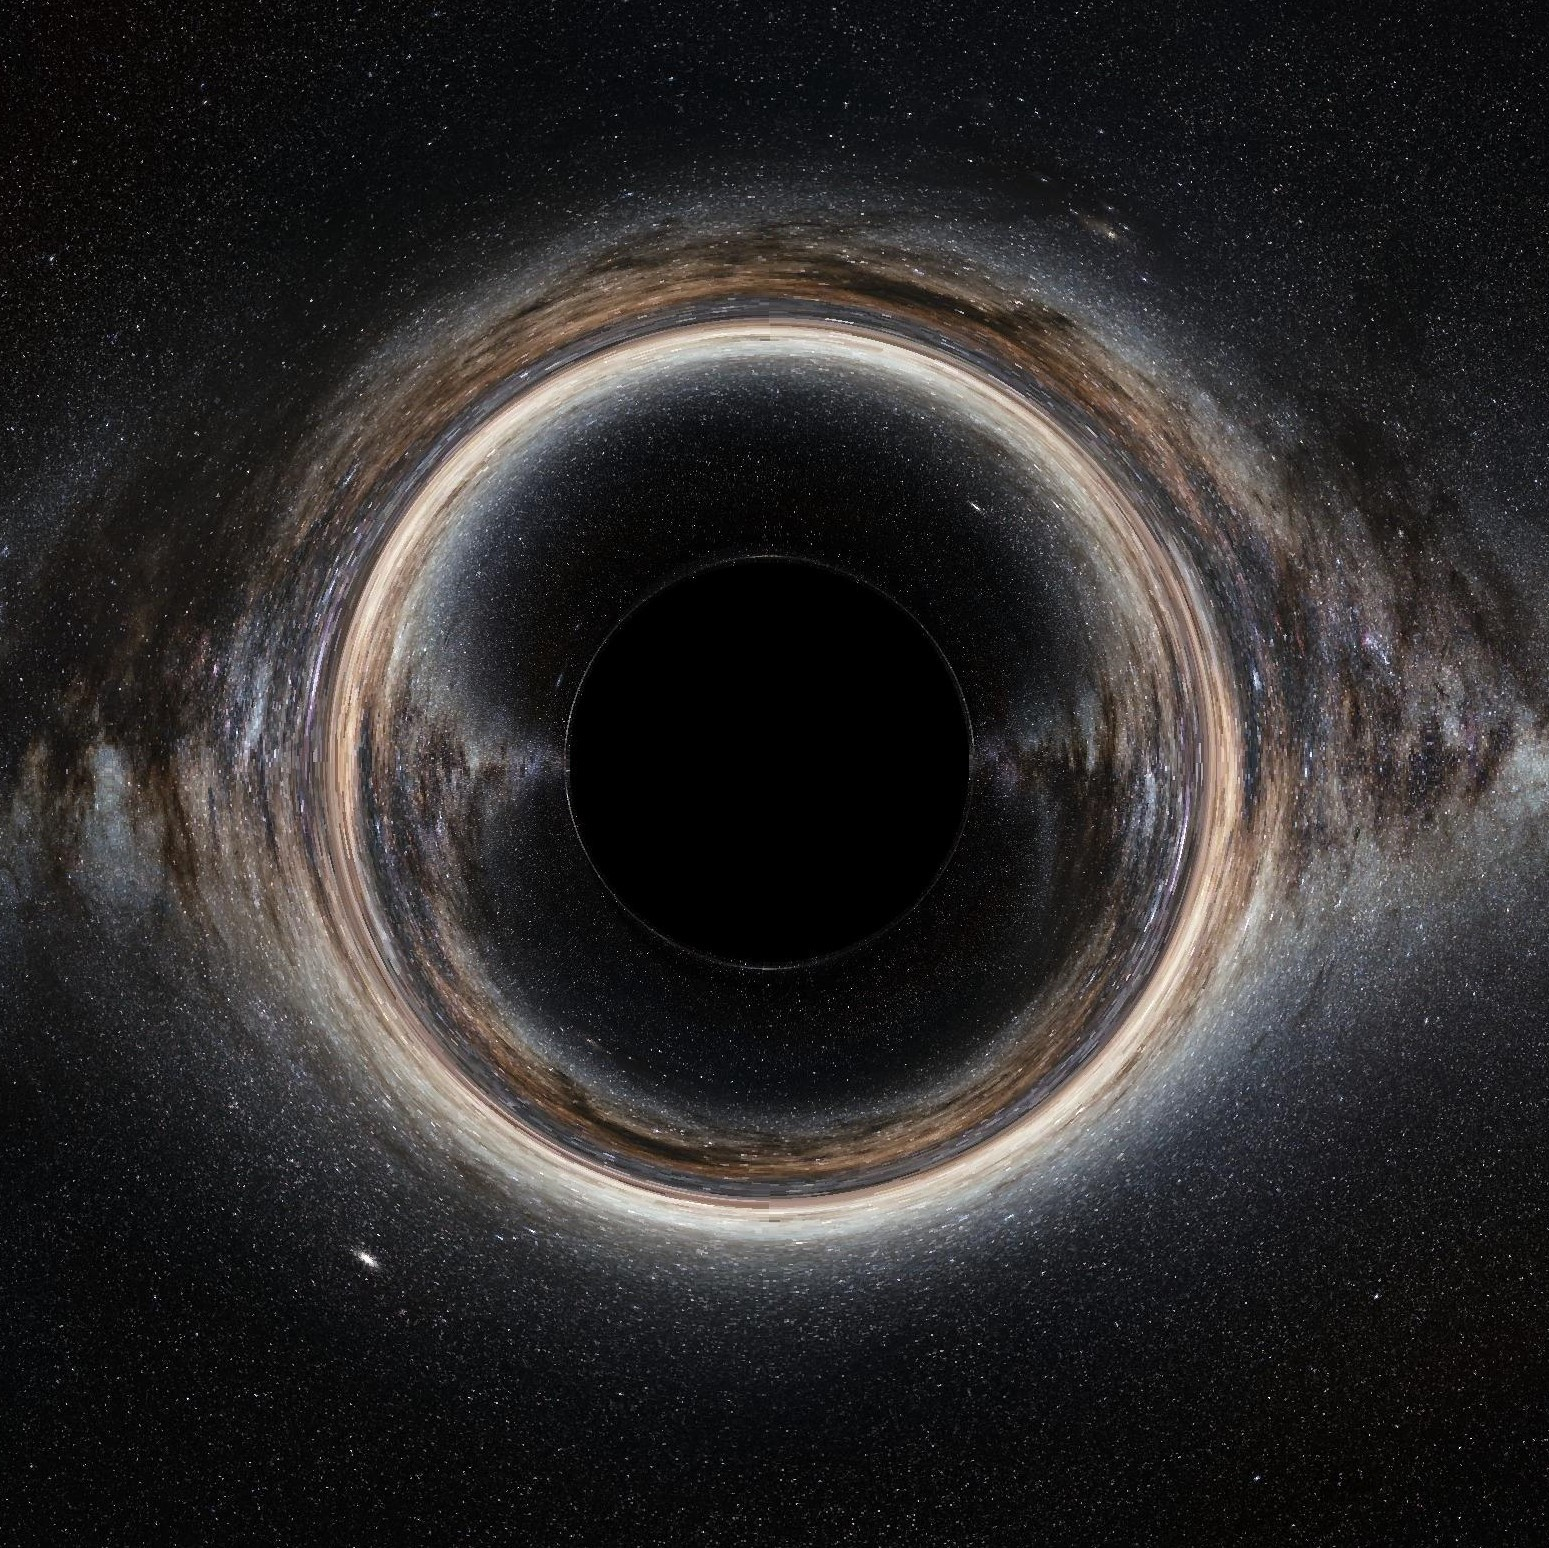
\includegraphics[height=0.45\linewidth]{hdri-pov(0)}
\captionof{figure}{An example of finding a pixels final position (left). 
A model of the shadow of a Schwarzschild black hole (right)}
\end{center}

Once a model of the shadow of a Schwarzschild black hole has been generated, there are many interesting things to analyse; however, all features seen here may also be seen in a Kerr black hole, and in section 5, many comments on Figure 4 apply to Figure 1 (right).
\end{multicols}
}

%----------------------------------------------------------------------------------------
%	The Kerr Metric
%----------------------------------------------------------------------------------------

\headerbox{3. The Kerr Metric}{name=kerr,column=0, span=2,below=introduction,above=references}{
\begin{multicols}{2}
Unlike the Schwarzschild metric, the Kerr metric is not spherically symmetric, meaning we cannot embed our equations into two dimensions. This is because the addition of angular momentum removes the arbitrary nature of $\theta$. Unfortunately this also means that the metric, and equations of motion associated with it, are significantly more complicated.

\vspace{1em}
In Boyer-Lindquist coordinates, a 'stretched' cartesian coordinates with the stretch factor determined by the amount of spin the metric has, the Kerr metric can be written as:

\begin{equation}
ds^{2} = -\left(1-\frac{2r}{r^2+a^2\mbox{Cos}^2(\theta)}\right) dt^2+\frac{r^2+a^2\mbox{Cos}^2(\theta)}{r^2-2r+a^2}dr^2+(r^2+a^2\mbox{Cos}^2(\theta))d\theta^2+
\end{equation}
\[ \left(r^2+a^2+\frac{2ra^2\mbox{Sin}^2(\theta)}{r^2+a^2\mbox{Cos}^2(\theta)}\right) \mbox{Sin}^2(\theta)d\varphi^2-\frac{4ra\mbox{Sin}^2(\theta)}{r^2+a^2\mbox{Cos}^2(\theta)}dtd\varphi \]

\vspace{1em}

One difference between a rotating black hole and a non-rotating black hole is that according to the general theory of relativity, a rotating black hole will collapse to a ring singularity, as opposed to a point singularity commonly thought of for a Schwarzschild black hole.

\vspace{1em}
By analysing this metric and the coefficients of certain components, we can find some key surfaces - notably the inner and outer event horizon and ergosphere:

\vspace{1em}
$\textbf{Event horizon}$

The event horizon of a black hole will be a familiar concept to most people; it is the area in which light cannot escape the black hole regardless of velocity (i.e the area in which escape velocity is infinite). To find the horizon(s) of the Kerr black hole, we look at when the coefficient of the radial component of the metric tends to infinity:

\begin{equation}
{r_{H}}^{\pm} = 1\pm\sqrt{1+a^2}
\end{equation}

\vspace{1em}
This gives us the positions of the inner and outer horizons respectively. Here the outer horizon would be known as the event horizon.
\vspace{2em}




$\textbf{Ergosphere}$

The ergoregion is one of the significant differences angular momentum introduces to a black hole. It is a region extending from the event horizon to some surface outside in which test particles cannot stay stationary, regardless of velocity, named the outer ergosphere. Another way of thinking about this is that the black hole is spinning so quickly near to the event horizon that the matter around it is rotating faster than the speed of light.

\vspace{1em}
By seeing when the coefficient of the temporal component of the metric changes sign, one may compute the radius of the inner and outer ergosphere:

\begin{equation}
{r_{E}}^{\pm} = 1\pm\sqrt{1-a^2\mbox{Cos}^2(\theta)}
\end{equation}

When the sign of the coefficient of the temporal component of the metric is negative, for a worldline to stay light-like, our photon must co-rotate sufficiently with the black hole. Since null geodesics are by definition light-like, they must satisfy this condition.

\begin{center}
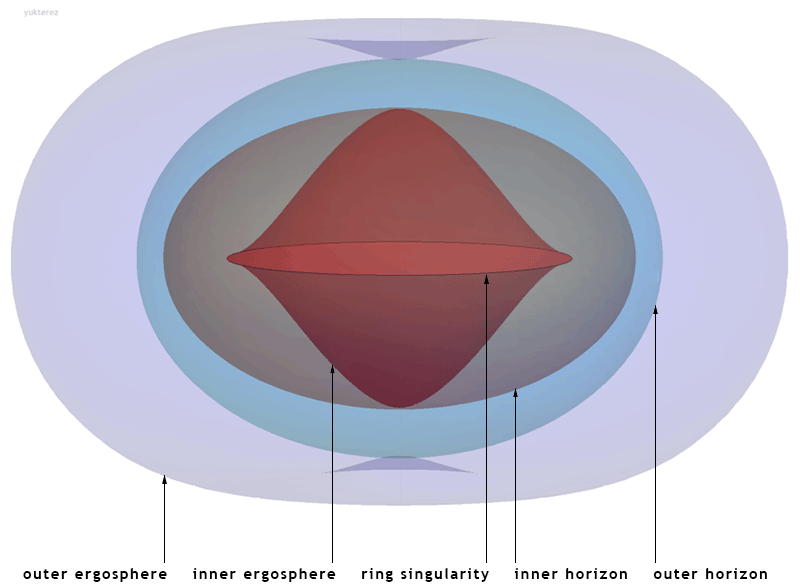
\includegraphics[width=0.7\linewidth]{Kerr-surfaces}
\captionof{figure}{Key surfaces of the Kerr metric \cite{yukterezKerr}}
\end{center}
\end{multicols}
}


%----------------------------------------------------------------------------------------
%	Modelling Photons in the Kerr Metric
%----------------------------------------------------------------------------------------

\headerbox{4. Modelling Photons in the Kerr Metric}{name=photons,column=2,row=0,below=schwarzschild,above=references}{

As in section 2, we may derive the equations of motion for light in the Kerr metric by looking at Hamiltonians formalisation and the conserved quantities implied by it, including; total energy, angular momentum in the axis of the black holes rotation and Carters constant.

\vspace{1em}
We end up with five coupled differential equations and many initial conditions determined by our input of r, $\theta$, $\varphi$, v and a. Here v is the initial velocity, and a = J = $\frac{J}{M}$ is the spin parameter for the black hole. We also take M = 1 for all black holes modelled as the mass is arbitrary - the importance is the ratio between inital distance from the centre of the black hole and the radius of the black hole - hence we can generalise and take M=1.

\vspace{1em}
Though rather crude, it is common practice in this field to treat the outer ergosphere as the outer horizon, and cut off all photon paths which enter the ergoregion. This is because very few photons can enter and have sufficient angular momentum to exit - so the effect on the realism of our image is minimal. Looking at Figure 3, we see the shape of the outer ergosphere being treated as the event horizon.

\vspace{1em}
Given certain initial conditions we may model a spherical orbit such as Figure 3. Spherical orbits have been studied extensively and their properties are well known \cite{teo2003spherical}.

\vspace{1em}
All coordinate choices for the Kerr metric come with their own issues - for Boyer-Lindquist this is the line $\theta = 0,\pi$ as we divide by zero along these lines. Solutions include discarding photon paths which pass through this line, or stitching two coordinate systems together, shifting to use a rotated Boyer-Lindquist coordinate system if any paths approach this axis.

\begin{center}
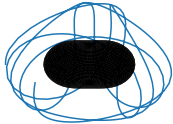
\includegraphics[width=0.4\linewidth]{3d-kerr-plot}
\captionof{figure}{A spherical photon path in the Kerr metric}
\end{center}
}


%----------------------------------------------------------------------------------------
%	Gravitational Lensing
%----------------------------------------------------------------------------------------

\headerbox{5. Gravitational Lensing}{name=lensing,column=3,row=0}{

\begin{center}
\includegraphics[width=0.75\linewidth]{milkyway-kerr-full-new(0)}
\captionof{figure}{A model of the gravitational lensing of a Kerr black hole}
\end{center}

\vspace{1em}
After generating an image like Figure 4, we may notice and analyse some important features:

\vspace{1em}
The shape of the shadow produced by the event horizon shifts from circular to being D-shaped as spin parameter is increased; this was famously originally proposed by Bardeen \cite{bardeen1973timelike} in 1973. The explaination for this is that photons fired towards the black hole with direction matching the spin gain energy; where some paths may have entered the event horizon in the Schwarzschild metric, in the Kerr metric they gain enough velocity to escape the gravitational pull. Conversely if a photon is travelling in the opposite direction it loses a significant amount of energy and is pulled into the event horizon.

\vspace{1em}
We also note the Einstein ring, made clear by my choice of celestial sphere in Figure 4. The Einstein ring is the ring of pixels whos final angle is the central pixel in our celestial sphere, meaning it is a ring of images of that which was directly behind the centre of the black hole in line with our start point. The Einstein ring in Figure 4 is in the middle of the ring showing the galaxy which is in the centre of our celestial sphere image, so it resembles a slightly squashed circle.

\vspace{1em}
Another key feature of all black holes is the secondary and tertiary (and so on) images which appear due to the infinite number of ways a photon can reach a point in space. We see a primary image for all points on the celestial sphere; this is the result of a photon path which has passed around the black hole but not orbited. We can also clearly see secondary images of some of the more obvious parts of the image near the black hole, coming from photon paths which have orbitted the black hole just once and reached their final position. If we had a perfect model, then near the flat left side of the black holes shadow, we would see repeated lines becoming thinner and thinner as we approach the edge; these being other paths of photons orbiting the black hole an arbitrary amount of times.
}

%------------------------------------------------



%----------------------------------------------------------------------------------------
%	Future Research
%----------------------------------------------------------------------------------------

\headerbox{6. Future Research}{name=future,column=3,row=0,below=lensing,above=references}{

In the future I would like to create a more realistic image of the gravitational lensing caused by a Kerr black hole. This involves accounting for some effects and objects that I have so far been ignoring:

\vspace{1em}
Accretion discs - In the real world, black holes almost certainly all have accretion discs; matter orbitting the black hole which the black hole 'feeds' off. I would like to take this into account in my imaging.

\vspace{1em}
Gravitational redshift - When light gains or loses velocity, it is shifted across the light spectrum and its intensity is changed. I am planning to keep track of velocity to implement this.

\vspace{1em}
The ergosphere - As previously mentioned, I am currently treating the outer ergosphere as a kind of pseudo event horizon. It would be preferable to more appropriately deal with photon paths which enter and exit the ergoregion.

\vspace{1em}
\begin{center}
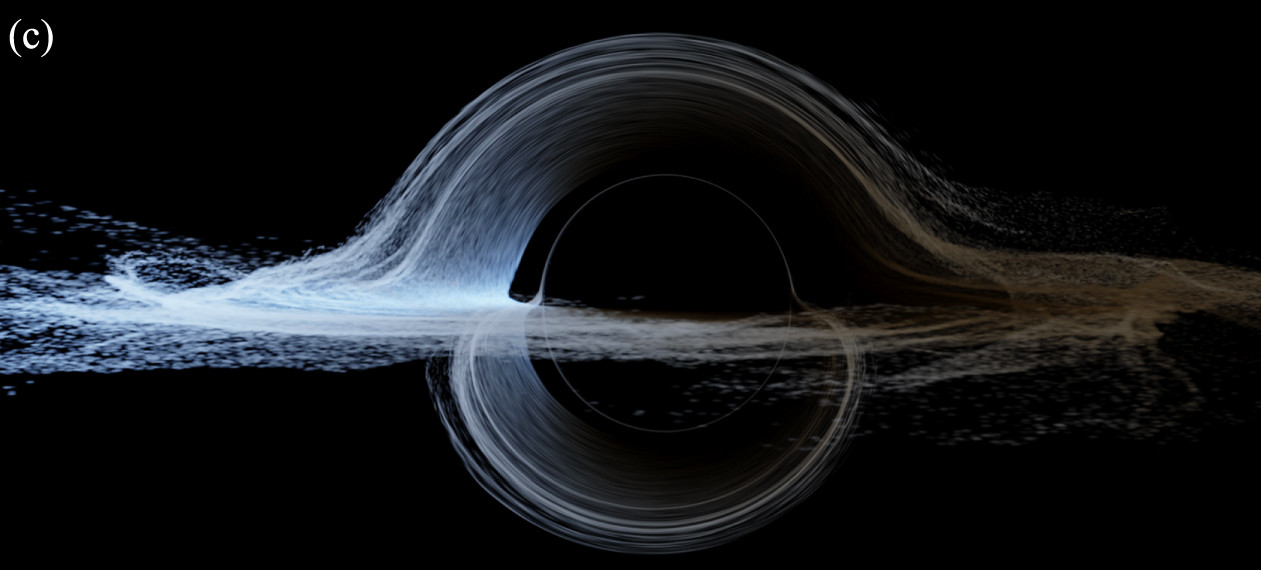
\includegraphics[width=0.65\linewidth]{realistic}
\captionof{figure}{A realistic model of a Kerr black hole \cite{james2015gravitational}}
\end{center}
}


\end{poster}

\end{document}